\section{Problem Description}

\begin{frame}{LMDD as MAPF}
    \begin{itemize}
        \item Tasks for each agent (drone) described by tuples:
        \[
        task_i \coloneq \{(x_{\text{start}_i}, y_{\text{start}_i}) , (x_{\text{goal}_i}, y_{\text{goal}_i})\}, \forall \text{ drone } d_i
        \]
        \item Grid bounds: $x \leq X, y \leq Y$.
        \item Goal: find paths $P_{d_i}$ making the path length as short as possible.
    \end{itemize}
\end{frame}

\begin{frame}{Path Planning and Constraints}
    \begin{itemize}
        \item Drones limited to four principal movements: upward $(x, y+1)$, downward $(x, y-1)$, rightward $(x+1, y)$, and leftward $(x-1, y)$.
        \item Adjacency: $(x_1,y_1)$ is adjacent to $(x_2,y_2)$ $\iff |x_2-x_1| + |y_2-y_1| = 1$.
        \item New decision variable: $t_{\text{begin}}$ (arrival time).
    \end{itemize}
\end{frame}

\begin{frame}{LMDD Goals}
    \begin{itemize}
        \item Given time $T$, minimize the sum of distances of all drones.
        \item Allow drones to wait in cells and choose entry time.
        \item Non-weighted distances make the problem easier than standard MAPF.
    \end{itemize}
\end{frame}

\begin{frame}{Network Flow Problem}
    \begin{itemize}
        \item MAPF is equivalent to multi-commodity minimum cost maximum flow problem \cite{lavalle}.
        \item Visualized as Network Flow problem.
        \item The number of drones is a max flow in the time-expanded net
    \end{itemize}
\end{frame}



\begin{frame}{MAPF as Network Flow Problem}
    \begin{itemize}
        \item Transformation into a time-expanded network  \cite{yu_timeoptimal}.
    \end{itemize}
    \begin{figure}[H]
        \centering
        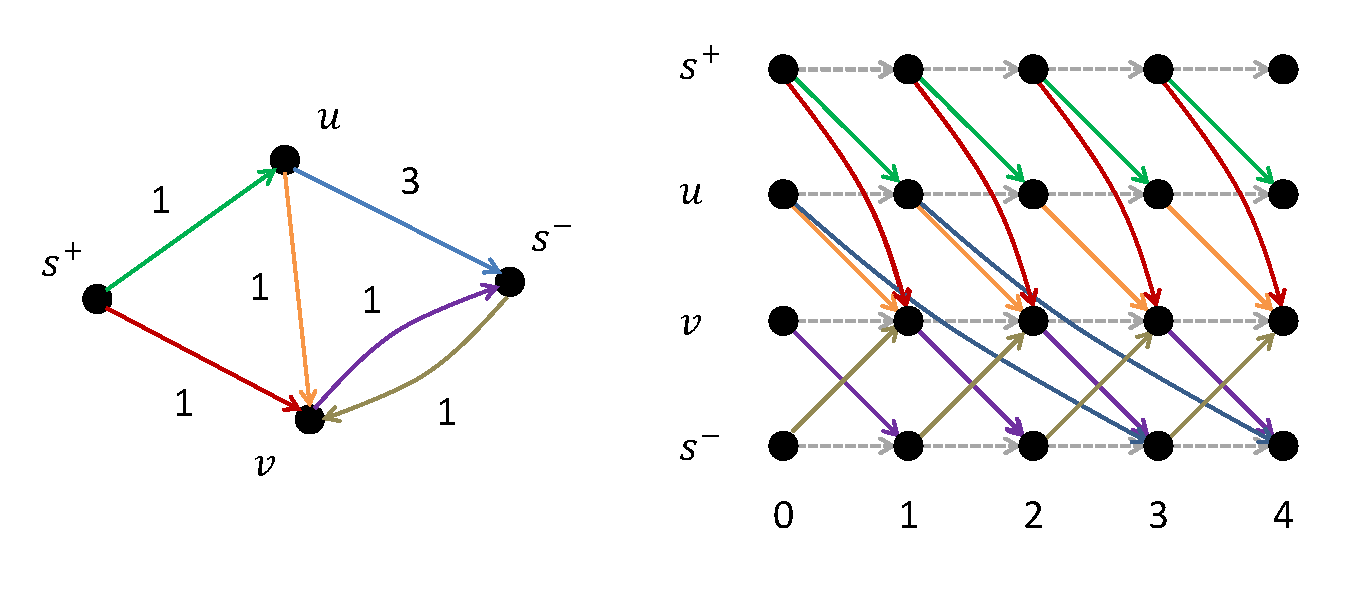
\includegraphics[width=0.8\textwidth]{img/time_extended_net_image.pdf}
        \caption{Time-expanded network representation (sourced from \cite{time_optimal_slides})}
        \label{fig:time_expanded_network}
    \end{figure}
\end{frame}

\begin{frame}{Multi-Commodity Flow Formulation}
    \begin{itemize}
        \item Each drone is a separate commodity flowing from start to goal node.
        \item Ensuring each drone reaches its goal within a given time horizon $T$.
    \end{itemize}
    \begin{figure}[H]
        \centering
        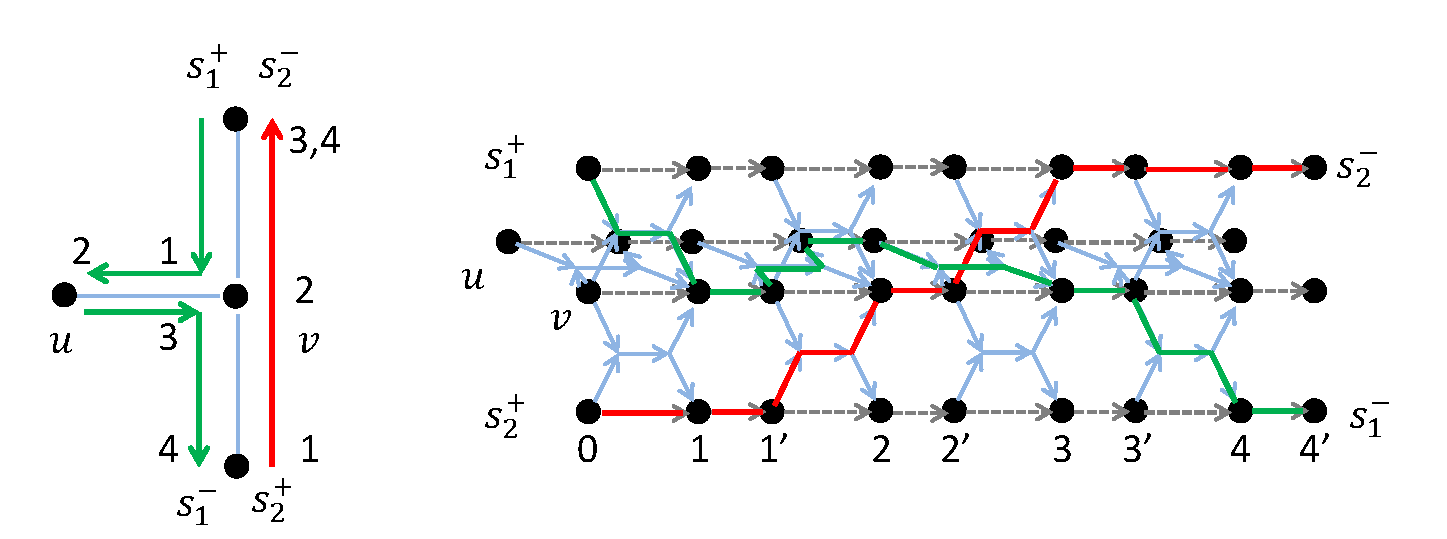
\includegraphics[width=0.8\textwidth]{img/equi_mapf_flow_image.pdf}
        \caption{Equivalence of MAPF to multi-commodity network flow (sourced from \cite{time_optimal_slides})}
        \label{fig:equi_mapf_flow}
    \end{figure}
\end{frame}

